%!TEX TS-program = xelatex
%!TEX encoding = UTF-8 Unicode

% Load Thesis Class
\documentclass{DEIThesis}

\title{Scheduling resources and managing HARQ retransmissions in Non-Terrestrial Networks}

\author{Francesco Rossato}
\studentId{2082121}

% Advisor
\advisor{Prof.\ Marco Giordani}

% If you are co-advised
\coadvisor{Dott. Matteo Pagin}
\coadvisorsUniversity{University of Padova}

\university{University of Padova}
\mastername{ICT for Internet and Multimedia}
\academicYear{2023/2024}

\begin{filecontents*}[overwrite]{\jobname.xmpdata}
    \Title{Scheduling resources and managing HARQ retransmissions in Non-Terrestrial Networks}
    \Author{Francesco Rossato}
    \Language{en-EN}
    \Keywords{ICT\sep ntn\sep non terrestrial networks \sep francesco rossato\sep LaTeX}
\end{filecontents*}

% Document

\begin{document}
    % The front matter (Cover, ToC, Abstract, etc...)
    \frontmatter

    % The main content
    \mainmatter
    %!TEX root = ../main.tex

\chapter{Introduction}
\label{chp:intro}

The term \ac{NTNs} denotes a category of networks where at least one link is routed via an aerial or space-borne vehicle such as \ac{HAPs}, \ac{UAVs} or telecommunication satellites.

\section{The focus on non-terrestrial networks}
The Third Generation Partnership Project \footnote{\href{https://www.3gpp.org}{\texttt{3gpp.org}}} (3GPP), the standardization body developing protocols for mobile communication networks, recently put a great emphasis on the importance of the integration of different access technologies along with the existing terrestrial mobile telecommunication infrastructure \cite{3gpp-tr-21.917}.

The envisioned future for mobile communications, starting with the already established 5G \ac{NR} and expanding with the new sixth-generation cellular networks (6G), foresees the integration of a non-terrestrial component. The latest \ac{3GPP} releases (Rel. 17 and Rel. 18) require 5G and 6G networks to be able to provide non-terrestrial satellite access complementing the already existing terrestrial access technologies \cite{overview-rel-17-18-saad} \cite{5g-nr-communication-geo-leo-maattanen}.

\section{Limitations of terrestrial networks}
The following paragraphs present a few scenarios where terrestrial networks have some limitations, and \ac{NTNs} can be used to provide connectivity.

\subsection{Remote places}
While \ac{TN} make the well-established foundation of today’s mobile communication infrastructure, their own nature poses some intrinsic limitations to their deployment in certain scenarios, especially in rural and remote areas. Conditions such as harsh terrain and geographical impediments act as natural barriers to the deployment of terrestrial infrastructure. Moreover, ground infrastructure requires the presence of an already established reliable power grid, driving up the costs that telecommunication companies would have to sustain.
The population density is often low in remote and rural places, so the already high infrastructure cost will hardly pay for itself, making this kind of market even more unattractive to private investors and further limiting the possibility for the people living there to access a resource which is becoming increasingly more important.

As studied and documented in \cite{6g-challenge-opportunity-base-pyramid}, the issue of an inadequate broadband coverage in rural regions is an enormous challenge, but also a great opportunity to kick-start the economy of currently underdeveloped countries, promoting a more fair access to the internet and alleviating the problem of digital divide between different parts of the world.

\subsection{Redundancy}
Another limitation of the current terrestrial infrastructure is the lack of redundancy and robustness against natural disasters. Extreme events such as earthquakes, fires and floods, but also deliberate behaviors such as targeted attacks by terrorist organizations and sabotages can disrupt the connectivity even for a long period of time, causing significant economical damage and hindering the already difficult rescue efforts, potentially leading to loss of lives.

The simple installation of a greater number of base stations is not a viable solution because they all share the same weaknesses.

In this scenario, \ac{NTNs} can act as redundant access methodology to decrease downtimes of terrestrial infrastructure, provide emergency communication services and also additional capacity when required. 

\subsection{Long distances and sensors}
Remote equipment, offshore plants and distribution grids will also benefit from the research carried out in this field, since providing terrestrial connectivity in those scenarios is a challenging task. The installation of an underwater optical fiber link to serve a single endpoint, such as an offshore power plant in the ocean, would bear a disproportional cost compared to the functions required, and maintenance would be another challenging and expensive task. 
The deployment of a non-terrestrial network would provide connectivity on a global scale, therefore allowing internet access in isolated places without the need for a dedicated connection.

Consider now the problem of connecting of a number of sensors placed in a large area. When distances are large, solutions may either be the densification of radio stations or the use of a lower frequency in order to have a less severe propagation loss. However, those approaches have their downsides and are not always feasible. In this case, the large coverage area of \ac{NTNs} will undoubtedly be useful to provide internet connection \cite{performance-ntn-support-iot-wang}.

\paragraph{} Other scenarios where \ac{NTNs} can become useful in overcoming the limitation of their terrestrial counterpart are well described in \cite{ntn-6g-era-challenges-giordani} and \cite{potential-multilayered-nierarchical-ntn-wang}.

\section{Satellite types}
Satellites are divided in three different categories depending on their orbiting altitude: \ac{GEO}, \ac{MEO} \ac{LEO} satellites. Each one has its own characteristics, as briefly described below.

\subsection{GEO satellites}
orbiting at 35.786Km, \ac{GEO} satellites appear stationary since their orbiting period is the same as the Earth rotation period. This vastly simplifies the tracking for the ground equipment, since once the position of the \ac{UE} is known, the relative position of the satellite is known, too.
    
Since \ac{GEO} satellites are geostationary, continuous coverage to a designated area can be provided using as little as a single satellite, while the use of non-\ac{GEO} satellites would require the deployment of a constellation, which is both more complex and more expensive.

Their higher altitude creates a large cell footprint, larger than both \ac{MEO} and \ac{LEO}, so the overall cost to provide coverage to the same area is lower.

The disadvantages of \ac{GEO} satellites are mainly linked to the large distance with the \ac{UE}: the transmission power and the antenna gain have to be higher to account for the greater propagation losses, and the propagation delay of the signal travelling at the speed of light is about 120ms, so if the \ac{UE} sends a request to a server at time zero through a \ac{GEO} link, the best-case delay will be of half a second without considering any protocol-related delay.

In addition to the positive aspects previously discussed, the larger cell footprint also means that a single satellite will be serving a massive number of users, so the total available capacity will have to be shared between a bigger number of actors, and the throughput experienced by each one of them will be reduced. 
Moreover, the high number of users leads to a large rate of initial access  requests, with the possibility of channel saturation as described in \cite{3gpp-tr-38.811}.

\subsection{LEO satellites}
Orbiting below the altitude of 2.000Km, \ac{LEO} satellites are the most promising solution in the realm of \ac{NTNs} for a number of reasons hereby discussed.
    
The lower altitude entails a shorter propagation delay, and the smaller coverage area of each satellite means that the total number of users that need to be served is smaller. 

The cost per satellite is significantly smaller than \ac{GEO} and \ac{MEO} satellites. However, given that they are not geostationary, a large constellation is needed to provide a continuous service, driving up the deployment costs significantly. As an example of those constellations, Fig. \ref{fig:starlink_constellation} depicts the \ac{LEO} satellites employed by Starlink\footnote{Starlink is a satellite internet constellation operated by Starlink Services, LLC, a wholly-owned subsidiary of American aerospace company SpaceX.}, with 4.808 units in service at the time of writing\footnote{Source: \href{https://satellitemap.space/}{\texttt{satellitemap.space}}}.

\begin{figure}[ht]
    \centering
    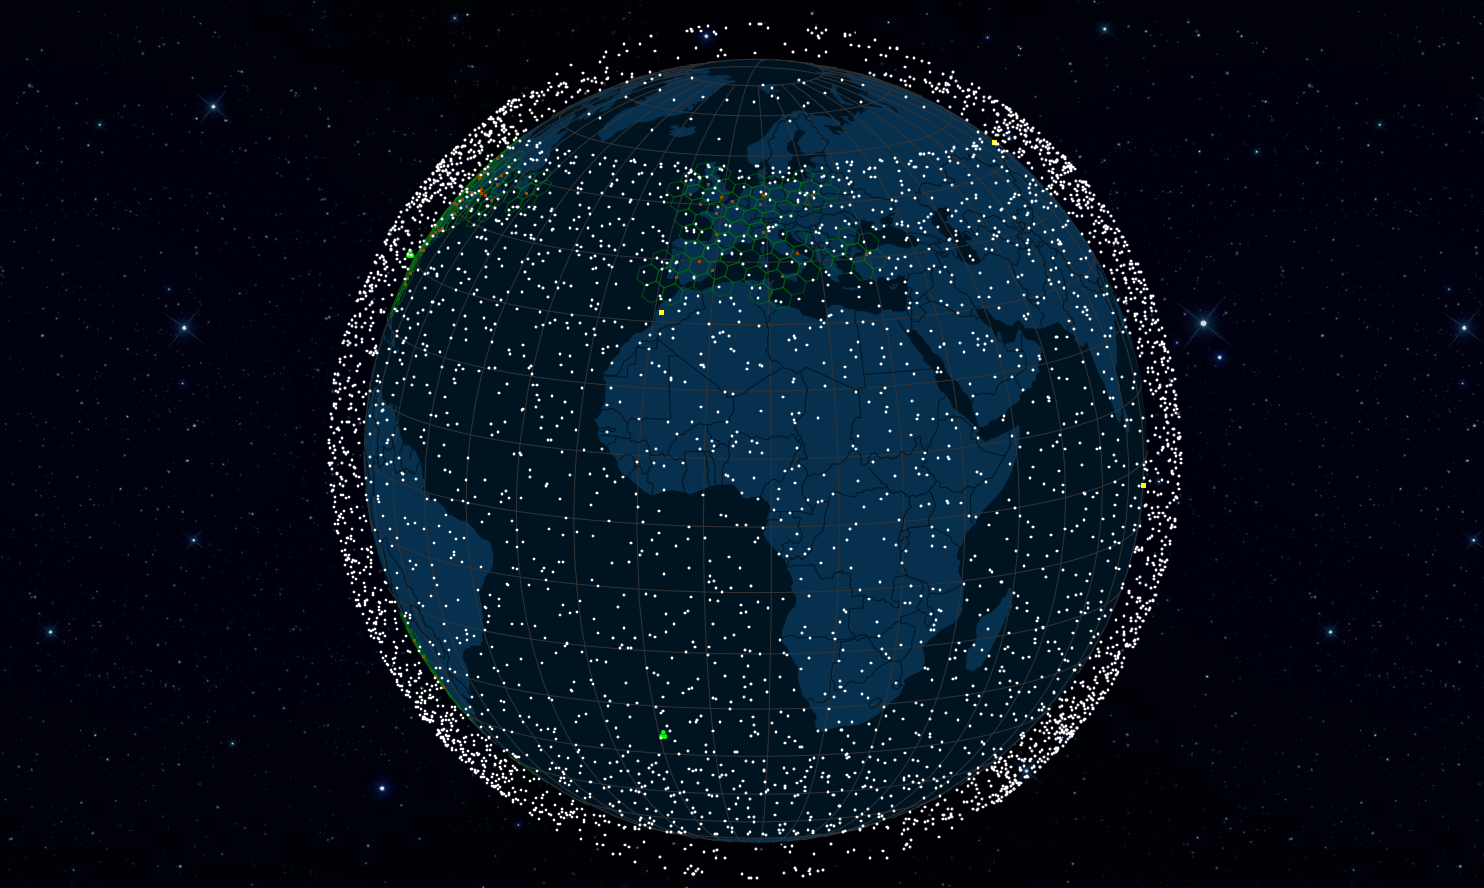
\includegraphics[width=0.7\textwidth]{res/starlink-constellation.png}
    \caption{Starlink constellation as July 2024. Source: \href{https://satellitemap.space/}{\texttt{satellitemap.space}}}
    \label{fig:starlink_constellation}
\end{figure}

The smaller altitude at which \ac{LEO} satellites orbit enables the use of higher frequency bands, since the experienced path loss is smaller compared to \ac{GEO} satellites. This in turn allows for higher throughput, as detailed in \cite{satellite-communication-mmwave-giordani}

The aforementioned solutions are not to be considered mutually exclusive. In fact, the multitude of possibilities that their combinations offer open to the study of various different scenarios, as detailed in \cite{potential-multilayered-nierarchical-ntn-wang}

\subsection{Current solutions}
Current solutions for non-terrestrial communication do exist, but they mostly rely on telecommunications satellites placed in the \ac{GEO}, at a height of 35.786 km. The distance that the signal has to travel offering limited throughput and large delays. While \ac{LEO} constellations (400 km to 2.000 km) have proven to be a valid alternative, providing higher throughput and lower latency \cite{main-features-5g-nr-ntn-yun}, they have the drawback of an increased Doppler shift due to their high speed relative to ground \cite{satellite-communication-mmwave-giordani}, and there is still no international standard with regard to the communication protocols to use. 

\paragraph{}
This scenario led \ac{3GPP} to identify some work to be done to integrate \ac{NTN} in cellular standards, calling for long-term research in this field \cite{satellite-communication-mmwave-giordani}. This work will mainly focus on the 

\paragraph{}\todo{move this to state of the art} Focusing on the \ac{MAC} sublayer, the large propagation delay of satellite links affects different aspects, making the actual implementation not suited for a \ac{NTN} scenario. In the \ac{HARQ} protocol, the retransmission timeout is likely to expire before a single \ac{RTT}, leading to unnecessary retransmissions. Moreover, the limit on the maximum number of concurrent \ac{HARQ} processes leads to a stop-and-wait behaviour, which may increase the energy consumption \cite{3gpp-tr-38.811}. On the other hand, it has been noted that disabling \ac{HARQ} would lead to an even worse performance penalty, therefore requiring a redesign for \ac{NTN} \cite{5g-beyond-5g-ntn-trends-vanellicoralli}. Another 5G \ac{NR} protocol which is negatively impacted in \ac{NTN} is the initial access, since users at the center of the cell face a smaller propagation delay with respect to users at the cell edge \cite{5g-beyond-5g-ntn-trends-vanellicoralli} \cite{applying-nr-technologies-in-ntn-lee}. As a result, preambles of \ac{UE}s placed near the cell edge may reach the satellite when the \ac{RACH} opportunity has already expired, which may lead to collisions. During the initial access phase, \ac{UE}s are not aware of their propagation delay, and the high mobility of \ac{gNB}s on \ac{LEO} satellites causes a non-negligible Doppler shift. Those factors vary with the relative position and speed between the \ac{UE} and the \ac{gNB}, and the protocols for initial access must be modified in \ac{NTN} to account for them \cite{ntn-from-5g-6g-hassan}. 
\paragraph{}
It is clear that the future of mobile networks envisioned by \ac{3GPP} embraces \ac{NTN}s, and considerable work has to be done. Research will bear a high impact towards a more connected, equal opportunity world. 

\section{Currrent state of the art}
\todo{types of payloads: regenerative, and transparent or bent pipe}
    \include{chapters/02_releated}
    %!TEX root = ../main.tex

\chapter{Background}
\label{chp:background}

\begin{algorithm}[ht]
    \caption{An algorithm with caption}\label{alg:two}
    \begin{algorithmic}
        \REQUIRE $n \geq 0$
        \ENSURE $y = x^n$
        
        \STATE $y \gets 1$
        \STATE $X \gets x$
        \STATE $N \gets n$
        
        \WHILE{$N \neq 0$}
            \IF{$N$ is even}
              \STATE $X \gets X \times X$
              \STATE $N \gets \frac{N}{2} $  \COMMENT{This is a comment}
            \ELSIF{$N$ is odd}
              \STATE $y \gets y \times X$
              \STATE $N \gets N - 1$
            \ENDIF
        \ENDWHILE
    \end{algorithmic}
\end{algorithm}

\begin{equation}
e^{j\pi} + 1 = 0
\end{equation}
    %!TEX root = ../main.tex

\chapter{HARQ}
\label{chp:analysis}

\section{Concurrent processes limit}

One of the problems highlighted by the \ac{3GPP} technical report \cite{3gpp-tr-38.811} on the matter of non-terrestrial networks regards the maximum number of concurrent \ac{HARQ} processes. 

\subsection{Processes explained}
The details of \ac{HARQ} protocol implementation in the 5G \ac{NR} standard is extensively treated in many publications such as \cite{harq-wireless-communications-survey}. However, for the purpose of understanding what is a harq process and how it affects the throughput in a non-terrestrial scenario, a brief overview of a few key concepts is enough.

\begin{figure}[ht]
    \centering
    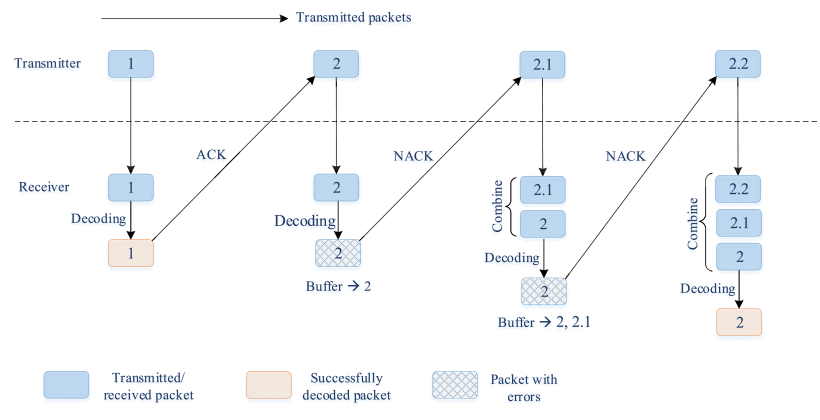
\includegraphics[width=0.7\textwidth]{res/harq-retx-scheme.png}
    \caption{\ac{HARQ} retransmission diagram \cite{harq-wireless-communications-survey}}
    \label{fig:harq_retx_scheme}
\end{figure}


\paragraph{}\ac{HARQ} is a stop-and-wait protocol, meaning that it is designed to wait for the arrival of previous packet's \ac{ACK} before sending the new one. While this enforces the delivery of ordered packets, it also brings the downside of severely underutilizing the channel capacity, wasting resources that could potentially be used for transmission instead \cite{3gpp-ts-38.214}.

This limitation can be overcome by the introduction of multiple concurrent processes.

A \ac{HARQ} process starts when a \ac{TB} is passed to the \ac{HARQ} entity and finishes when the \ac{ACK} relative to that same \ac{TB} is received by the sender. After the \ac{ACK} is correctly received, the next \ac{TB} starts being processed. Considering a link with propagation delay $\tau_p$, the minimum active time for a process is therefore $2\tau_p$. 

5G \ac{NR} standard allows the base station to configure the maximum number of concurrent \ac{HARQ} processes each user can have, with the default value being 8 and the maximum 16 \cite{3gpp-ts-38.300}. 

\paragraph{Example} Consider an example scenario where each process tries to send a \ac{TB} at the maximum possible rate, every $2\tau_p$, to a \ac{LEO} satellite orbiting at 2.000Km, therefore having $\tau_p\approx6$ms. Assuming the best possible conditions with no need for retransmissions and assuming that the base station grants the \ac{UE} to the best possible clearance of 16 concurrent processes, the total send rate is of 16 transfer blocks every 12ms. In order to target a throughput of 50Mbps, the block size must therefore be of at least $$\frac{\textit{target throughput} \times 2\tau_p}{\textit{number of processes}} = 37,5Kb$$

This is not a realistic option even for terrestrial networks, where the \ac{SNR} poses a less stringent constraint, let alone for non-terrestrial ones.


\todo{Problem of harq concurrent processes: each process has a timeout of 100ms and the max number of processes is 100. A higher number of concurrent processes crashes the simulator. As the propagation delay increases and the sending interval decreases, we are forced to keep more harq processes concurrently active, therefore reducing the number of leftover slots for additional processes. Once we reach the critical value of 100, any other packet will crash the simulator.
So, as we increase the throughput, we must also increase the number of harq processes, since there are mote packets concurrently in flight.}

\todo{investigate the latency problem at 13ms propagation delay}
\todo{explain how harq works}
    %!TEX root = ../main.tex

\chapter{Conclusions and Future Works}
\label{chp:conclusions}

This work has provided a comprehensive study on the impact that the high propagation delay experienced in \ac{NTN}s has in layer-2 protocols. The current codebase of the ns-3 network simulator has been properly extended to allow for end-to-end simulation of the \ac{NR} stack in a \ac{NTN} scenario, since the ns-3 implementation of \ac{NR} technology was not designed for high propagation delays. A lot of work went therefore into the design, implementation, and testing of a base support for the simulation of \ac{NTN}s.

It was shown that propagation delay plays a crucial role in the performances of \ac{NR} in \ac{NTN}s, affecting both the efficiency and reliability of data transmission.

\paragraph{}
Once the simulator was ready, focus has been placed on the optimization of the \ac{HARQ} protocol in \ac{NTN}s, investigating its shortcomings when delaing with large propagation delays as well as proposing some original solutions to increase its performances.

\section{Results}
\subsection{Simulator redesign}
Since the state of the art in network simulation tools was not ready for complete \ac{NR} \ac{NTN} simulations, presenting numerous problems especially at the scheduler, a redesign of certain behaviors was performed.

\subsubsection{Scheduling with propagation delay}
This study has found (section \ref{sec:pd-sched-acc}) that the current scheduling with short advance (i.e. scheduling only a slot in advance: at time $t_0$ the schedule allocates the resources of time $t_0+1$ms) does not work in \ac{NTN} because the propagation delay itself is longer than the delay between the act of scheduling and the time for which the scheduling happens. 

The proposed solution uses information on the propagation delay to adjust the advance of the scheduling process. 

\subsubsection{BSR timer}

Another flaw discovered in the implementation of current \ac{NR} protocols in \ac{NTN} involves the periodic \ac{BSR} that the \ac{UE} keeps sending every 10ms (section \ref{sec:bsr-timer}). 

While this approach presents some (undesired) benefits, it is not the intended behavior, therefore the current implementation, albeit working, is far from an ideal choice.

The proposed solution consists of adapting the \ac{BSR} timer accordingly to the propagation delay, never allowing it to assume values smaller than a round-trip time. 

\subsubsection{Inflated BSR}
If the interval between the packets generated by the application is smaller than the \ac{RTT}, each \ac{BSR} will report the whole size of the transmission buffer, even though other \ac{SR} relative to packets already present in the buffer may be still in-flight. While leading to an overall lower latency, this vastly increases the amount of resources being wasted, since the \ac{UE} will find itself with many unnecessary transmission grants (Section \ref{sec:inf-bsr}).

The proposed solution is to limit the scheduling requests that are triggered every time a packet arrives into the transmission buffer to the new data only.

\subsubsection{Reordering timer}
The conducted simulation campaigns have found that anytime a packet is fragmented and sent across multiple frames, a reordering and recomposition timer is activated at the \ac{gNB} side, which, however, is too short with respect to the large propagation delay in \ac{NTN}s, expiring before all the pieces of the packet have the chance to arrive (Section \ref{sec:reord-timer}).

The implemented solution was to extend such timer in order to account for the propagation delay.

\subsection{HARQ}
\subsubsection{Concurrent processes}
This work confirmed that the 16 maximum concurrent \ac{HARQ} processes allowed per user heavily limits the achievable throughput (section \ref{sec:harq-conc-proc}).

Different solutions have been proposed, including completely disabling the protocol as well as increasing the number of allowed concurrent processes.

Both these solutions have also been implemented in the simulator, evaluating scenarios with no \ac{HARQ}, then 16, 32, 64 and 100 maximum concurrent processes. 

It was found that increasing the number of processes allows for considerably higher throughputs, while disabling \ac{HARQ} is only feasible in conditions of high \ac{SNR}.

Since having \ac{HARQ} enabled still proved to be helpful in a scenario of low \ac{SNR}, a more aggressive version of \ac{HARQ} was designed, where each process was allowed to send two packets instead of one before waiting for the \ac{ACK}. This solution managed to roughly double the achievable throughput with respect to the standard \ac{HARQ} implementation.

\section{Future work}

The preparation of this work required many simulations to be run and evaluated, and as expected some design problems emerged. With a thoughtful approach, each unexpected behavior was investigated and solutions were devised, implemented and tested.

While effort was made to provide more than a single solution, striving to look at the problems from different perspectives to find more than a single way to approach it, some possibilities still require a deeper study, and some observations were made whenever it was felt that a point might benefit from additional work.

This section describes some possible future paths that might have the potential to improve the solutions proposed in this work, as well as different approaches which performances are still to be evaluated.

\paragraph{}
The current behavior of waiting for packets to arrive at the transmission buffer of the \ac{UE} before transmitting the \ac{SR} to the \ac{gNB} harshly impacts the experienced latency, since in the best-case scenario it at least adds a round-trip time of delay. While this is not a problem in terrestrial networks because base stations are relatively close to the \ac{UE}s that are serving, in \ac{NTN}s the added delay is noticeable. 

A predictive algorithm capable of visualizing patterns in the \ac{UE}-generated traffic, forecasting its behavior in the immediate future and preemptively sending \ac{SR} so that new packets will be able to be transmitted right away without additional delays would be of invaluable help in reducing the overall latency of the link.

\paragraph{}
Timers often represent a trade-off between higher performances and a more robust network. This is the reason behind the proposal of a dynamic approach when setting the values for \ac{BSR} periodic requests and reordering timer. Since the delay of \ac{NTN}s can experience large variations depending on the satellite orbit, configurable timers shall be preferred instead of using fixed values.

\paragraph{}
Regarding \ac{HARQ}, a dynamic way of enabling and disabling it on the fly based on channel quality indicators could be beneficial, since it was shown that high-\ac{SNR} scenarios performed better with \ac{HARQ} disabled, while conditions of low \ac{SNR} benefitted from having it enabled.

\paragraph{}

It is clear that further research is needed to develop more effective strategies for managing propagation delay in \ac{NTN}s. This includes exploring new technologies, improving existing methodologies, and devising innovative network architectures.

Ultimately, this work aims to pave the way for future research and practical applications in the field of \ac{NTN}s, emphasizing the need for continuous innovation and adaptation to meet the evolving demands of modern communication systems. 

The findings of this thesis not only contribute to the existing body of knowledge on \ac{NTN}s but also pave the way for future research in this evolving field.

    
    % Bibliography, appendix, acknowledges, etc...
    \backmatter
\end{document}